  \documentclass[crop]{standalone}% 'crop' is the default for v1.0, before it was 'preview'
%\usetikzlibrary{...}% tikz package already loaded by 'tikz' option
\usepackage[utf8]{inputenc}

\usepackage[dvipsnames]{xcolor}
\usepackage{tikz}
\usetikzlibrary{
  arrows,
automata,
backgrounds,
calc,
decorations.pathreplacing,
fit,
petri,
positioning,
shadows,
shapes,
snakes,
}


\begin{document}

  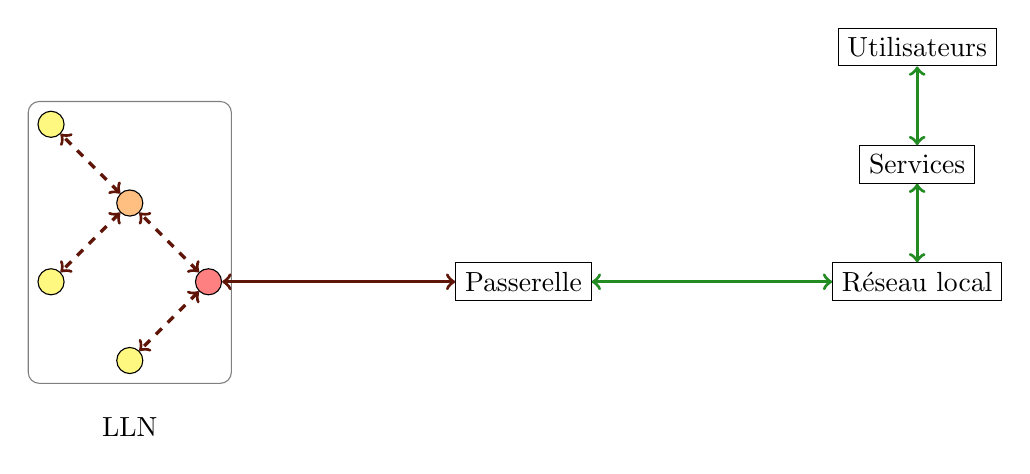
\begin{tikzpicture}

  % définition des styles
  \tikzstyle{visible}=[draw, fill=blue!50]
  \tikzstyle{hidden}=[ draw, fill=gray!20]
  \tikzstyle{router}=[circle, draw, fill=orange!50,text=black]
  \tikzstyle{child}=[circle, draw, fill=yellow!50,text=black]
  \tikzstyle{root}=[circle, draw, fill=red!50,text=black]

  % les nœuds
  \node[draw] (gw) {Passerelle};

  % \node[draw, below=of gw] (topology) {Topologie réseau connue?};
  % \node[draw, below left=of topology] (noinfo) {Estimation ``étoilée''};
  % \node[draw, below right=of topology] (route) {Estimation ``maillée''};

  % Réseau contraint
  \node[root] (1) at (-4, 0) {};
  \node[router] (2) at (-5, 1) {};
  \node[child] (3) at (-5, -1) {};
  \node[child] (4) at (-6, 2) {};
  \node[child] (5) at (-6, 0) {};

  % \node[cloud, cloud puffs = 10, minimum width = 4cm, draw, fill = gray!10] (cloud) at (5,0) {Réseau local};
  \node[draw] (cloud) at (5,0) {Réseau local};

  \node[draw, above=of cloud] (service) {Services};
  \node[draw, above=of service] (users) {Utilisateurs};

 \node [fit=(1) (2) (3) (4) (5), rounded corners, draw=black!50] (lln) {};
 \node [below=.3 cm of lln] {LLN};

\path

  % Réseau contraint
  (gw) edge[<->, very thick, Sepia] (1)
  % (1) edge[<->, very thick, bend left=20, ForestGreen] (2)
  % (1) edge[<->, very thick, bend left=20, ForestGreen] (3)
  % (2) edge[<->, very thick, bend left=20, ForestGreen] (4)
  % (2) edge[<->, very thick, bend left=20, ForestGreen] (5)

  (1) edge[<->, very thick, dashed, Sepia] (2)
  (1) edge[<->, very thick, dashed, Sepia] (3)
  (2) edge[<->, very thick, dashed, Sepia] (4)
  (2) edge[<->, very thick, dashed, Sepia] (5)


  % Réseau conventionnel
  (gw.east) edge[<->, very thick, ForestGreen] (cloud)
  (service) edge[<->, very thick, ForestGreen] (cloud)
  (service) edge[<->, very thick, ForestGreen] (users)
  % % Cache
  % (gw) edge[->,very thick] (topology)
  % (topology) edge[->, very thick] node [midway, above left] {Non} (noinfo.north east)
  % (topology) edge[->, very thick] node [midway, above right] {Oui} (route.north west)
  ;

  \end{tikzpicture}
  \end{document}